\documentclass[a4paper, 11pt]{article}

\usepackage[utf8]{inputenc}
\usepackage[T1]{fontenc}
\usepackage[super]{natbib}
\usepackage[french]{babel}
\usepackage{helvet}
\usepackage[top=35mm, bottom=35mm, left=25mm, right=25mm]{geometry}
\usepackage{geometry}
\usepackage{graphicx}
\usepackage{multirow}  
\usepackage{subfigure}
\usepackage{verbatim}
\usepackage{url}
\usepackage{algorithm2e, algorithmic} 
\usepackage{amsmath,amsfonts,amssymb}
\usepackage{lmodern}
\usepackage{microtype}
\usepackage{xcolor}
\usepackage{textcomp}
\usepackage{minted}
\usepackage{framed}
\usepackage{tcolorbox}
\usepackage{wrapfig}
\usepackage{etoolbox}
\BeforeBeginEnvironment{minted}{\begin{tcolorbox}[left=8mm]\begin{center}}
\AfterEndEnvironment{minted}{\end{center}\end{tcolorbox}}%
\usepackage{hyperref}
\hypersetup{
pdfpagemode={},
pdfstartview={XYZ 3000 3000 0.75}
pdfstartview={XYZ left top zoom}
}
\hypersetup{
pdftitle={M1 ISICG - Introduction au Traitement Numérique des Images},
pdfsubject={Rapport de projet},
pdfauthor={Rouijel Mehdi},
pdfkeywords = {M1, ISICG, Traitement, Images, Numérique, Université de Limoges, Faculté des Sciences et Techniques}
}
\setcounter{secnumdepth}{3}

\usepackage{fancyhdr}
%\pagestyle{fancy}
% \lhead{}
% \rhead{}
\fancypagestyle{plain}{%
\fancyhf{} % clear all header and footer fields
\fancyfoot[C]{\fontfamily{\familydefault}\fontsize{10pt}{14pt}\selectfont page \thepage} % except the center
\renewcommand{\headrulewidth}{1pt}
\renewcommand{\footrulewidth}{1pt}}
\pagestyle{plain}


\renewcommand{\familydefault}{phv}
%\renewcommand{\familydefault}{\sfdefault}

\definecolor{unilim_blue}{HTML}{103147}
\definecolor{unilim_red}{HTML}{9e3232}

\hypersetup{
    colorlinks,
    citecolor=unilim_red,
    filecolor=unilim_red,
    linkcolor=unilim_red,
    urlcolor=unilim_red,
}

\renewcommand{\thesection}{\color{unilim_red}\textsc\Roman{section}}
\renewcommand{\thesubsection}{\color{unilim_red}\textsc\thesection-\Roman{subsection}}


\begin{document}

%
%  -------
% | TITLE |
%  -------
%

\begin{titlepage}
\setlength{\headheight}{0cm}
\setlength{\headsep}{0cm}
{
  \noindent
  \begin{tabular}[t]{@{}l}
    \small\textsc{Université de Limoges}\\
    \small{Faculté des Sciences et Techniques}
  \end{tabular}
  \hfill
  \begin{tabular}[t]{l@{}}
    \small{Année Universitaire 2016 - 2017}
  \end{tabular}
  
  \vspace{-5.5mm}
  \begin{figure}[!h]
	\hspace*{-7.5mm}
\includegraphics[height=20mm]{img/unilim-fst.jpg}
  \end{figure}
      
  \vspace{20mm}
  \begin{center}
    
    \large\underline{Master \textsc{Informatique} ISICG, semestre 2}\\
    \Large\textsc{traitement numérique des images}
    
    \vspace{15mm}
  
    \begin{tcolorbox}[colback=unilim_blue, colframe=unilim_blue, boxrule=0.5pt, arc=4pt,
                      left=6pt, right=6pt, top=6pt, bottom=6pt, boxsep=0pt]
      \begin{minipage}[h]{\linewidth}
        \begin{center}
        { \color{white}
          \vspace*{5mm}
          \huge\textsc{Détection de Cibles de Fléchettes}\\
          \vspace*{5mm}
          \Large\textbf{\underline{Rapport de projet}}
          \vspace*{5mm}
        }
        \end{center}
      \end{minipage}
    \end{tcolorbox}
    
    \vspace{2mm}
    
    \large{version du \today}
    \vspace{25mm}\\
    Auteur\\~\\
    {
    \large
    \bsc{Rouijel} Mehdi
    }
    
  \end{center}
  
  \vfill
  \begin{flushleft}
	Responsable  : M. \bsc{Crespin} Benoît\\
  \end{flushleft}
}
\end{titlepage}

\clearpage


%
%  ---------
% | CONTENT |
%  ---------
%

\section*{\color{unilim_red}\textsc{Introduction}}
\paragraph{}
L'objectif de ce projet est de mettre en pratique les notions vues en cours, en particulier la transformée de Hough, en créant une application capable de détecter une cible de fléchettes dans une image. Au delà de la simple détection de la cible, le programme devrait pouvoir reconnaître ses différentes zones ainsi que les numéros autour; si des fléchettes sont présentes dans l'images, elles devraient être détectées aussi, pour éventuellement être capable de déterminer le score.

\bigskip

\section{Utilisation de l'application}
\paragraph{}
Une fois l'application lancée depuis Eclipse, une image par défaut est chargée. Pour utiliser une autre image, il suffit de naviguer vers \og File > Open... \fg{} pour sélectionner une nouvelle image. Il est aussi possible de sauvegarder l'image qui est vue dans la partie droite de la fenêtre, après avoir exécuté une opération, en utilisant \og File > Save... \fg{}. La copie (\og Edit > Copy \fg{}) n'est pas implémentée.
\paragraph{}
Chaque bouton du panneau de contrôle est indépendant. Par exemple, il est possible de n'appliquer que le flou, mais c'est l'image originale, et non le résultat de celui-ci, qui sera utilisée si la détection des contours est appliquée ensuite.\par
Différents paramètres peuvent être changés, en ouvrant la barre d'options du panneau de contrôle, pour la détection de contours, la détection de lignes et la détection d'ellipses. Elle sont expliquées dans la suite de ce rapport.

\section{Détection des contours}
\paragraph{}
\begin{wrapfigure}{r}{0.35\textwidth}
\vspace{-4mm}
\centering
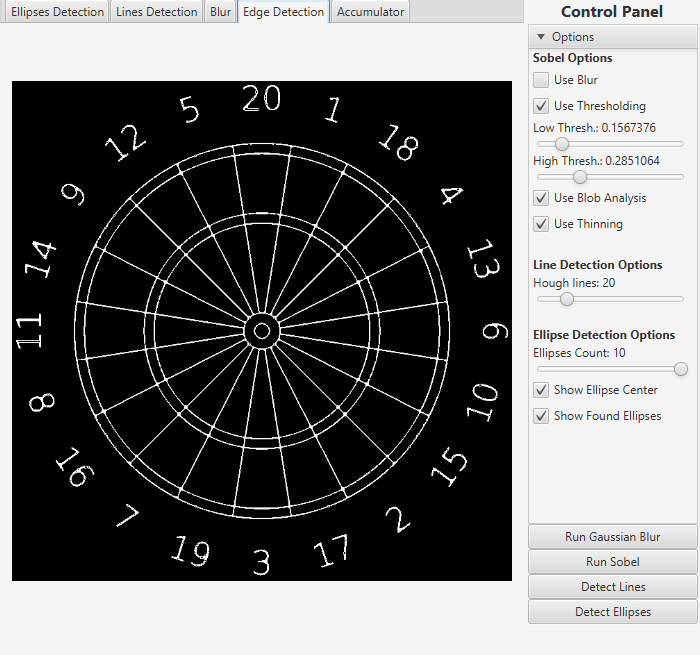
\includegraphics[width=0.35\textwidth]{img/front_edges_00.png}
\vspace{-8mm}
\caption{Contours trouvés}
\label{fig:frontEdges00}
\end{wrapfigure}
La détection des contours se fait par une application du filtre de Sobel qu'il est possible d'améliorer grâce aux différentes options disponibles dans le panneau de contrôle. Sélectionner l'ensemble des options rapproche le traitement d'un filtre de Canny \cite{wiki_canny}, avec dans l'ordre :
\begin{itemize}
\item Réduction du bruit par un filtre de Gauss
\item Seuillage
\item Analyse de région (\og blob analysis \fg{})
\item Amincissement
\end{itemize}
Il est à noter que deux seuils peuvent être modifiés. Le seuil haut concerne l'étape de seuillage et détermine la valeur frontière pour séparer les pixels affichés des pixels de fond. Le seuil bas est utilisé par l'analyse locale ; celle-ci ne pourra d'ailleurs fonctionner que si le seuillage est aussi sélectionné.\par
Lors de l'étape de seuillage, les pixels au-dessus du seuil haut sont marqués comme \og forts \fg{} et les pixels entre les deux seuils sont marqués comme \og faibles \fg{}. Par la suite, un pixel faible ne sera gardé que s'il est connecté à un pixel fort. En fonction de l'image, on peut constater une amélioration du résultat.

\section{Détection des lignes}
\paragraph{}
\begin{wrapfigure}{r}{0.35\textwidth}
\vspace{-4mm}
\centering
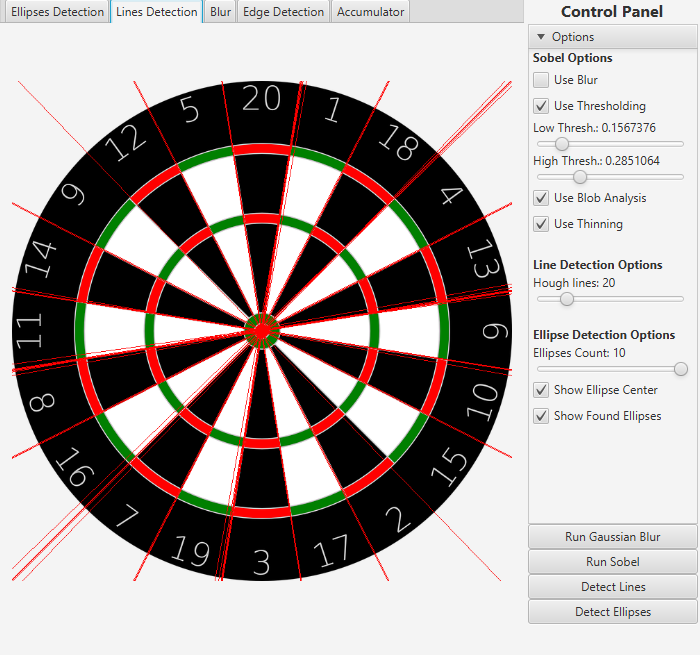
\includegraphics[width=0.35\textwidth]{img/front_lines_00.png}
\vspace{-8mm}
\caption{Lignes trouvées}
\label{subfig:frontLines00}
\end{wrapfigure}

\section{Détection des ellipses}
\paragraph{}
\begin{figure}[!h]
\centering
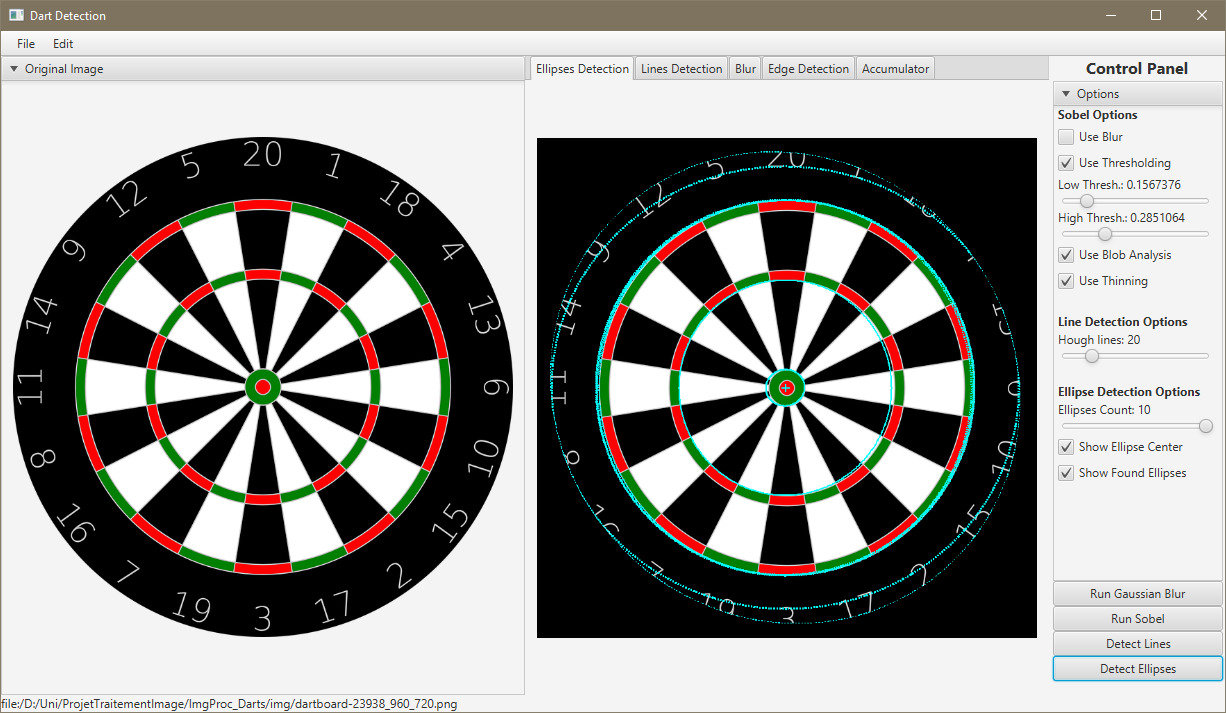
\includegraphics[width=0.85\linewidth]{img/front_result_00.png}
\vspace{-3mm}
\caption{Résultat de la détection d'ellipses avec \ref{fig:frontEdges00} et \ref{subfig:frontLines00}}
\label{fig:frontResult00}
\end{figure}

\bigskip

\section*{\color{unilim_red}\textsc{Conclusion}}
\subsection*{Travail non réalisé}

\subsection*{Aller plus loin}

\clearpage
  

\nocite{*}


%
%  --------------
% | BIBLIOGRAPHY |
%  --------------
%

\bibliographystyle{plain}
\bibliography{M1_TraitementImages_ROUIJEL}


\end{document}
